% Metódy inžinierskej práce

\documentclass[10pt,twoside,slovak,a4paper]{article}

\usepackage[slovak]{babel}
%\usepackage[T1]{fontenc}
\usepackage[IL2]{fontenc} % lepšia sadzba písmena Ľ než v T1
\usepackage[utf8]{inputenc}
\usepackage{graphicx}
\usepackage{url} % príkaz \url na formátovanie URL
\usepackage{hyperref} % odkazy v texte budú aktívne (pri niektorých triedach dokumentov spôsobuje posun textu)

\usepackage{cite}
%\usepackage{times}

\pagestyle{headings}

\title{Vplyv násilnych hier na správanie človeka\thanks{Semestrálny projekt v predmete Metódy inžinierskej práce, ak. rok 2022/23, vedenie: Ing. Vladimír Mlynarovič, PhD.}} % meno a priezvisko vyučujúceho na cvičeniach

\author{Adam Kačmár\\[2pt]
	{\small Slovenská technická univerzita v Bratislave}\\
	{\small Fakulta informatiky a informačných technológií}\\
	{\small \texttt{xkacmara@stuba.sk}}
	}

\date{\small 23. október 2022} % upravte



\begin{document}

\maketitle

\begin{abstract}
Článok sa zaoberá násilím vo videohrách a jeho vplyvom na hráčov počas hrania v online svete ako aj v reálnom živote. Bežný stereotyp rodičov detí v mladom veku, ktorý počul každý hráč pri hraní strieľačiek nám predostiera otázku či tomu tak naozaj je. Herný svet v dnešnej dobe ponúka množstvo variácií hier, ktoré nás dostávajú do pozícií vojakov, nájomných vrahov či obrancov vesmíru. Takéto široké spektrum nám ponúka aj možnosť herného zážitku pre viacerých hráčov a kompetitívny mód, pri ktorom sa dokáže hráč rozčúliť nad slabším výkonom spoluhráča či tímu a dá im to ľudovo „zožrať“. Pri veľkej dávke súťaživosti a vžitia sa do hry rastie rovnako aj agresia hráča. Otázkou tohto článku je či takáto agresia je vyvolaná práve typom hry, ktorá násilie podsúva. Výsledky nám dávajú štúdie, ktoré merali správanie účastníkov pri viacerých scenároch.
\end{abstract}



\section{Úvod}

V dnešnej dobe býva bežnou praxou, že sú videohry súčasťou voľného času mladých ľudí, pri ktorých sa odpútajú od reality počas hier s priateľmi. Počas dekád vývoja herného priemyslu sa vyvinuli žánre a herná realita do nepredstaviteľných rozmerov, u ktorých si ľudia v minulosti nedokázali predstaviť realizáciu. V posledných 15 rokoch takého technológie stúpli na nový výkonnostný level reality a s tým sa aj hry variabilných žánrov vykryštalizovali do absolútnej dokonalosti.

Jednými zo žánrov sú aj akčné a first-person shooter hry, ktoré sú založené na najmä na násilí voči nepriateľom v rôznych formách. Priamoúmerne s vývojom a modernizáciou videohier sa vizuálne približujú aj „strieľačký“ bližšie k reálnemu svetu. Pri týchto hrách je bežná herná možnosť módu pre viacerých hráčov, resp. multiplayer, v ktorom sa súťaživá nenávisť voči protihráčom premieňa na nenávisť z frustrácie voči spoluhráčov, ktorých výkon nenapĺňa ideálne predstavy hráča. Podobným nenávistným a násilným prejavom dokáže čeliť aj rodina a okolie hráča, v zriedkavých prípadoch aj udalosti, ktoré pohnú spoločnosťou, štátom aj svetom.  V minulosti sa spoločnosť stretla práve s touto otázkou pri masových vraždách, streľbách alebo teroristických činoch, za ktorými stáli mladí ľudia, u ktorých sa domnievalo, že dôležitým faktorom boli aj násilné videohry, ktoré pridávali myšlienky konateľom smrteľných aktov ~\ref{minulost}. Práve tieto korelácie medzi násilnými hrami, ktoré sledujú výskumy v posledných rokoch dávajú lepší drobnohľad na túto problematiku(~\ref{vyskum}). Záverečne poznámky podávajú pohľad individuála a laika ako aj samostatný výsledok výskumu.

%Motivujte čitateľa a vysvetlite, o čom píšete. Úvod sa väčšinou nedelí na časti.

%Uveďte explicitne štruktúru článku. Tu je nejaký príklad.
%Základný problém, ktorý bol naznačený v úvode, je podrobnejšie vysvetlený v časti~\ref{nejaka}.
%Dôležité súvislosti sú uvedené v častiach~\ref{dolezita} a~\ref{dolezitejsia}.
%Záverečné poznámky prináša časť~\ref{zaver}.


\section{Príčiny násilia a nenávisti} \label{priciny}


Z obr.~\ref{f:rozhod} je všetko jasné. 

\begin{figure*}[tbh]
\centering
%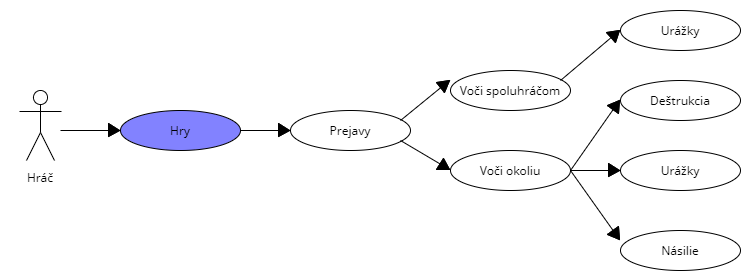
\includegraphics[scale=1.0]{diagram.pdf}
Aj text môže byť prezentovaný ako obrázok. Stane sa z neho označný plávajúci objekt. Po vytvorení diagramu zrušte znak \texttt{\%} pred príkazom \verb|\includegraphics| označte tento riadok ako komentár (tiež pomocou znaku \texttt{\%}).
\caption{Rozhodujúci argument.}
\label{f:rozhod}
\end{figure*}



\section{Prejavy násilia a nenávisti} \label{prejavy}

Prejavy násilia a nenávisti sú bežnou praxou počas hrania videohier. Takéto prejavy sa diferencujú aj podľa typu danej hry na offline hry a online hry. Každa subkategória má u svojich hier rôzne prejavy násilia a nenávisti, ktoré vznikajú frustráciou z priebehu hry, výkonov hráča alebo spoluhráčov alebo iných faktorov. Frustrácia pôsobí aj pri neschopnosti hráča ovládať hru správne alebo neschopnosti zlepšovať sa v nej\cite{UoR-Failure}, kde to bývajú prevažne offline hry. Pri online hrách sa pretláča aj nenávisť voči spoluhráčom, na ktorú poukazuje pasáž ~\ref{ina:spoluhraci}.

Môže sa zdať, že problém vlastne nejestvuje\cite{Coplien:MPD}, ale bolo dokázané, že to tak nie je~\cite{Czarnecki:Staged, Czarnecki:Progress}. Napriek tomu, aj dnes na webe narazíme na všelijaké pochybné názory\cite{PLP-Framework}. Dôležité veci možno \emph{zdôrazniť kurzívou}.


\subsection{Prejavy voči spoluhráčom} \label{ina:spoluhraci}
Prejavy nenávisti pri móde pre viacerých hráčov sú bežnou praxou pri videohrách. Hráč počas hrania prichádza do mnohých situácií, kde je dôležitá kooperácia so spoluhráčmi, ktoré môžu výrazne ovplyvniť priebeh hry. V prípade neúspechu a zlyhania jednotlivca sa dostávajú hráči do vzájomných sporov o tom, kto chybu spôsobil. 

\subsection{Prejavy voči okoliu} \label{ina:okolie}

Niekedy treba uviesť zoznam:

\begin{itemize}
\item jedna vec
\item druhá vec
	\begin{itemize}
	\item x
	\item y
	\end{itemize}
\end{itemize}

Ten istý zoznam, len číslovaný:

\begin{enumerate}
\item jedna vec
\item druhá vec
	\begin{enumerate}
	\item x
	\item y
	\end{enumerate}
\end{enumerate}

\paragraph{Veľmi dôležitá poznámka.}
Niekedy je potrebné nadpisom označiť odsek. Text pokračuje hneď za nadpisom.

\section{Regulácia okolím} \label{regulacia}


\section{Udalosti v minulosti} \label{minulost}



\section{Výskum} \label{vyskum}



\section{Záver} \label{zaver} % prípadne iný variant názvu



%\acknowledgement{Ak niekomu chcete poďakovať\ldots}


% týmto sa generuje zoznam literatúry z obsahu súboru literatura.bib podľa toho, na čo sa v článku odkazujete
\bibliography{literatura}
\bibliographystyle{plain} % prípadne alpha, abbrv alebo hociktorý iný
\end{document}
